\acused{GP}
Gaussian Processes (GPs) are a Bayesian method for regression. We consider the regression input
to be real-valued scalars $x_i$ and the regression output $f(x_i)=y_i$ as the value of a
function $f$ at $x_i$. The complete training data will be denoted by column
vectors $\mathbf{x}$ and $\mathbf{y}$. Unseen test input is denoted with
$\xprime$.
\ac{GP}s present a non-parametric way to express prior knowledge on the space of all possible functions $f$ modeling
a regression relationship.
Formally, a GP is an infinite-dimensional extension of the multivariate Gaussian distribution.

The collection of random variables $\br{f(x_i)=y_i}$ (indexed by $i$) represents the
values of the function $f$ at each location $x_i$.
We write $f \sim \mathcal{GP}(\mu,k \mid \thetabf_\text{mean},\thetabf)$, where
$\mu$ is the {\em mean function} and $k$ is the {\em covariance function} or {\em kernel}.
That is, $\mu(x_i \mid \thetabf_\text{mean})$ is the prior mean of the random variable $y_i$, and
$k(x_i,x_j \midtheta)$ is the prior covariance of the random variables $y_i$
and $y_j$. The output of both mean and covariance function are conditioned on a
few free hyper-parameters parameterizing $k$ and $\mu$. We refer to these
hyper-parameters as $\thetabf$ and
$\thetabf_\text{mean}$
respectively.
To simplify the calculation below, we will assume the prior mean $\mu$ is identically zero; once the derivation is done, this assumption can be easily relaxed via translation.
We use upper case
italic $K(\xbf,\xprime \midtheta )$ for a function that returns a matrix of dimension $I \times J$
with entries $k(x_i,x_j \midtheta )$ and with $x_i \in \xbf$ and $x_j \in
\xprime$ where $I$ and $J$ indicate the length of the column vectors $\xbf$ and
$\xprime$.
Throughout, we write $\Kbf_{(\thetabf,\xbf,\xprime)}$ for the prior covariance
matrix that results from computing  $K(\xbf,\xprime \midtheta )$. In the
following, we will sometimes drop the subscript $\xbf,\xprime$, writing
only $\Ktheta$, for clarity. Note that we do this only in cases when both
input vectors are identical and correspond to training input $\xbf$.
We differentiate two different situations leading to different ways samples can be generated with
this setup:
\begin{enumerate}
\item ${\yprime}$ - the predictive posterior sample from a distribution
conditioned on observed input $\xbf$ with observed output $\ybf$ and conditioned on
$\thetabf$.
\item $\ystar$ - a sample from the predictive prior. We will describe
situations, where the \ac{GP} has not seen any data $\xbf,\ybf$ yet. In this
case, we sample from a Gaussian distribution with 
     $\ystar \sim \mathcal{N}\big(0,K(\xstar, \xstar \midtheta
)\big)$; where the symbol $*$ indicates that no data has been observed yet. 
\end{enumerate}

We now show how to compute the predictive posterior distribution of test output $\yprime := f(\xprime)$ conditioned on training data $\ybf := f(\xbf)$.  (Here $\xbf$ and $\xprime$ are known constant vectors, and we are conditioning on an observed value of $\ybf$.) The predictive posterior can be computed by first forming the joint density when both training and test data are treated as randomly chosen from the prior, then fixing the value of $\ybf$ to a constant.  To start, let
\[
  \Sigma := \bmat{
    K(\xbf, \xbf \midtheta )     & K(\xbf, \xprime \midtheta )     \\
    K(\xprime, \xbf \midtheta ) & K(\xprime, \xprime \midtheta )
  }
  \text{ and }
  \Sigma^{-1} =: \bmat{
    \Mbf_{11} & \Mbf_{12} \\
    \Mbf_{21} & \Mbf_{22}
  }.
\]
We then have
\[
  P(\ybf, \yprime \midtheta )
  \propto
  \exp\br{
    -\frac12
    \bmat{\ybf^\top & \yprimetop}
    \bmat{\Mbf_{11} & \Mbf_{12} \\ \Mbf_{21} & \Mbf_{22}}
    \bmat{\ybf \\ \yprime}
  }.
\]
Treating $\ybf$ as a fixed constant, we obtain
\[
  P\pn{\yprime \mvert \ybf,\thetabf}
  \propto
  P(\ybf, \yprime \midtheta )
  \propto
  \exp\br{
    -\frac12 \yprimetop \Mbf_{22} \yprime
    - \hbf^\top \yprime
  },
\]
where $\hbf = M_{21} \ybf$ is a constant vector.  Thus $P(\yprime | \ybf,
\thetabf)$ is Gaussian,
\begin{equation}\label{eq:pred_posterior}
  P\pn{\yprime \mvert \ybf, \thetabf} \sim \Ncal(\mupost,
\Kbf_{\thetabf}^\text{post}),
\end{equation}
with covariance matrix $\Kpost = \Mbf_{22}^{-1}$.  To find its mean $\mupost$,
we note that $P_{\yprime|\ybf,\thetabf}(\yprime + \mupost)$ is Gaussian with
the same covariance as $P(\yprime | \ybf,\thetabf)$, but its exponent has no linear term:
\begin{align*}
  P_{\yprime|\ybf,\thetabf} \pn{\yprime + \mupost \mvert \ybf,\thetabf}
  &\propto
  \exp\br{
    -\frac12 (\yprime + \mupost)^\top \Mbf_{22} (\yprime + \mupost)
    - \hbf^\top (\yprime + \mupost)
  } \\
  &\propto
  \exp\br{
    -\frac12 \yprime\top \Mbf_{22} \yprime
    - \underbrace{(\hbf + \Mbf_{22} \mupost)^\top}_{\text{must be $0$}} \yprime
  }.
\end{align*}
Thus $\hbf = -\Mbf_{22} \mupost$ and $\mupost = -\Mbf_{22}^{-1} \hbf =
-\Mbf_{22}^{-1} \Mbf_{21} \ybf$.

The partioned inverse equations (\citealp*{barnett1979matrix} following \citealp*{mackay1998introduction}) give
\begin{align*}
  \Mbf_{22} &= \big(K(\xprime,\xprime \midtheta ) - K(\xprime,\xbf \midtheta ) K(\xbf,\xbf \midtheta )^{-1}
K(\xbf,\xprime \midtheta )\big)^{-1}, \\
  \Mbf_{21} &= -\Mbf_{22} K(\xprime,\xbf \midtheta ) K(\xbf,\xbf \midtheta )^{-1}.
\end{align*}
Substituting these in the above gives
\begin{align}
  \Kpost &= K(\xprime,\xprime \midtheta ) - K(\xprime,\xbf \midtheta )
K(\xbf,\xbf \midtheta )^{-1} K(\xbf,\xprime \midtheta ),\label{eq:K_hat} \\
  \mupost &= K(\xprime,\xbf \midtheta ) K(\xbf,\xbf \midtheta )^{-1}\ybf.\label{eq:mu_hat}
\end{align}
Together, $\mupost$ and $\Kpost$ determine the computation of the predictive posterior
with unseen input data (\ref{eq:pred_posterior}).

Often one assumes the observed regression output is noisily measured, that is,
one only sees the values of $\ybf_\noisy = \ybf + \wbf$ where $\wbf$ is
Gaussian white noise with variance $\sigma_\noise^2$. This noise term can be
absorbed into the covariance function $K(\xbf,\xbf \midtheta)$.
The log-likelihood of a \ac{GP} can then be written as:
\begin{equation}
\label{eq:gplogdens}
\log P(\ybf \mid \xbf,\thetabf) =
-\frac12 \ybf^\top 
\Ktheta^{-1} \ybf
- \frac12\log \abs{\Ktheta}
- \frac{n}{2}\log 2\pi
\end{equation}
where $n$ is the number of data points.
Both log-likelihood and predictive posterior can be computed efficiently using a \ac{SP} in Venture~\citep{mansinghka2014venture}
with an algorithm that resorts to Cholesky factorization~\citep[chap. 2]{rasmussen2006gaussian}.
We write the Cholesky factorization as 
$\Lbf\coloneqq \text{chol}(\Ktheta)$ when
:
\begin{equation}
\Ktheta = \Lbf\Lbf^\top
\end{equation}
where $\Lbf$ is a lower triangular matrix. This allows us to compute the inverse of a covariance matrix as
\begin{equation}
\Ktheta^{-1} = (\mathbf{L}^{-1})^\top (\mathbf{L}^{-1})
\end{equation}
and its determinant as 
\begin{equation}
det(\Ktheta) = det(\mathbf{L})^2
\end{equation}
We compute (\ref{eq:gplogdens}) as
\begin{equation}
\log(P(\ybf \mid \xbf, \thetabf)\coloneqq - \frac{1}{2} \ybf^\top \bm{\alpha} - \sum_i \log \mathbf{L}_{ii} - \frac{n}{2} \log 2 \pi
\end{equation}
where 
\begin{equation}
\label{eq:chol_L}
\mathbf{L} \coloneqq \text{chol}(\Ktheta)
\end{equation}
and 
\begin{equation}
\label{eq:alpha}
\bm{\alpha} \coloneqq  \mathbf{L}^\top \backslash(\mathbf{L} \backslash \ybf). 
\end{equation}
%This results in a computational complexity of $\mathcal{O}(n^3)$ in the number of data points for
%sampling with a complexity of $n^3/6$ for (\ref{eq:chol_L}) an $n^2/2$ for (\ref{eq:alpha}). 
This results in a computational complexity for sampling in the number of data points of $O(n^3/6)$ for (\ref{eq:chol_L}) an $O(n^2/2)$ for (\ref{eq:alpha}). 
Above, we defined the \ac{GP} prior as $\ystar \sim
\mathcal{N}\big(0,K(\xbf_*,\xbf_* \midtheta )\big)$.
We see that this prior is fully determined by its covariance function.
%%%%%%%%%%%%%%%%%%%%%%%%%%%%%%%%%%%%%%%%%%%%%%%%%%%%%%%%%%%%
%%%%%%%%%%%%%%%%%%%%%%%%%%%%%%%%%%%%%%%%%%%%%%%%%%%%%%%%%%%%
%%%%%%%%%%%%%%%%%%%%%%%%%%%%%%%%%%%%%%%%%%%%%%%%%%%%%%%%%%%%
\subsection{Covariance Functions}
The covariance function (or kernel) of a \ac{GP} governs high-level properties
of the observed data such as smoothness or linearity. The high-level properties
are indicated with superscript on functions.  A linear covariance can be written as:
%%%%%%%%%%%%%%%%%%%%%%%%%%%%%%%%%%%%%%%%%%%%%%%%%%%%%%%%%%%%
\begin{equation}\label{eq:LIN1}
    \klin =   \sigma_1^2(x x^\prime).
\end{equation}
%%%%%%%%%%%%%%%%%%%%%%%%%%%%%%%%%%%%%%%%%%%%%%%%%%%%%%%%%%%%
We can also express periodicity:
%%%%%%%%%%%%%%%%%%%%%%%%%%%%%%%%%%%%%%%%%%%%%%%%%%%%%%%%%%%%
\begin{equation}\label{eq:PER1}
    \kper =  \sigma_2^2 \exp \bigg( \frac{2 \sin^2 ( \pi (x - x^\prime)/p}{\ell^2} \bigg). 
\end{equation}
%%%%%%%%%%%%%%%%%%%%%%%%%%%%%%%%%%%%%%%%%%%%%%%%%%%%%%%%%%%%
By changing these properties we get completely different prior behavior for sampling $\ystar$ from a
\ac{GP} with a linear kernel
%%%%%%%%%%%%%%%%%%%%%%%%%%%%%%%%%%%%%%%%%%%%%%%%%%%%%%%%%%%%
\[
\ystar \sim \mathcal{N}\big(0,\Klin(\xstar,\xstar \mid \sigma_1 )\big)
\]
%%%%%%%%%%%%%%%%%%%%%%%%%%%%%%%%%%%%%%%%%%%%%%%%%%%%%%%%%%%%
as compared to sampling from the prior predictive with a periodic kernel (as depicted in 
Fig. \ref{fig:composition_tutorial} (c) and (d))
%%%%%%%%%%%%%%%%%%%%%%%%%%%%%%%%%%%%%%%%%%%%%%%%%%%%%%%%%%%%
\[
\ystar \sim \mathcal{N}\big(0,\Kper(\xstar,\xstar \mid \sigma_2, \ell )\big).
\]
%%%%%%%%%%%%%%%%%%%%%%%%%%%%%%%%%%%%%%%%%%%%%%%%%%%%%%%%%%%%
%%%%%%%%%%%%%%%%%%%%%%%%%%%%%%%%%%%%%%%%%%%%%%%%%%%%%%%%%%%%
\begin{figure}
 \centering

     \begin{subfigure}[b]{0.45\textwidth}
        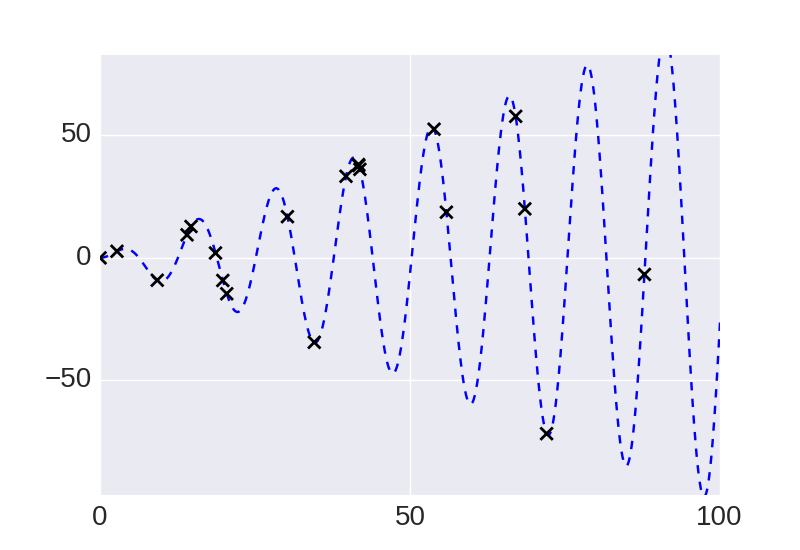
\includegraphics[width=\textwidth]{figs/composition/composition_demo_raw_data.png}
        \caption{Raw Data}
    \end{subfigure}
    ~ %add desired spacing between images, e. g. ~, \quad, \qquad, \hfill etc. 
      %(or a blank line to force the subfigure onto a new line)
    \begin{subfigure}[b]{0.45\textwidth}
\small
     \begin{align*}
    \text{LIN} &=   \sigma_1^2(x x^\prime)\\
    \text{PER} &=  \sigma_2^2 \exp \bigg( \frac{2 \sin^2 ( \pi (x - x^\prime)/p}{\ell^2} \bigg)\\ 
    \text{LIN} \times \text{PER} &=  \sigma_1^2(x x^\prime)\, \sigma_2^2 \exp \bigg( \frac{2 \sin^2 ( \pi (x - x^\prime)/p}{\ell^2} \bigg) 
    \end{align*}\vspace{5mm} 
        \caption{Kernels}
    \end{subfigure}\vspace{4mm} 


Parameterized Kernels:\vspace{3mm} 

     \begin{subfigure}[b]{0.3\textwidth}
      \centering \footnotesize
       $20.1^2(x x^\prime) $ \vspace{2mm}
	\caption{LIN}
    \end{subfigure}
    ~ %add desired spacing between images, e. g. ~, \quad, \qquad, \hfill etc. 
      %(or a blank line to force the subfigure onto a new line)
    \begin{subfigure}[b]{0.3\textwidth}
      \centering \footnotesize
      $19.1^2 \exp \bigg( \frac{2 \sin^2 ( \pi (x - x^\prime)/37.7}{6.3^2} \bigg)$ 
	\caption{PER}
    \end{subfigure}
    ~ %add desired spacing between images, e. g. ~, \quad, \qquad, \hfill etc. 
    %(or a blank line to force the subfigure onto a new line)
    \begin{subfigure}[b]{0.3\textwidth}
    \centering \footnotesize
      $383.9^2 (x x^\prime) \exp \bigg( \frac{2 \sin^2 ( \pi (x - x^\prime)/37.7}{6.3^2} \bigg)$ 
        \caption{LIN $\times$ PER}
    \end{subfigure} \vspace{4mm} 

Prior:

     \begin{subfigure}[b]{0.3\textwidth}
        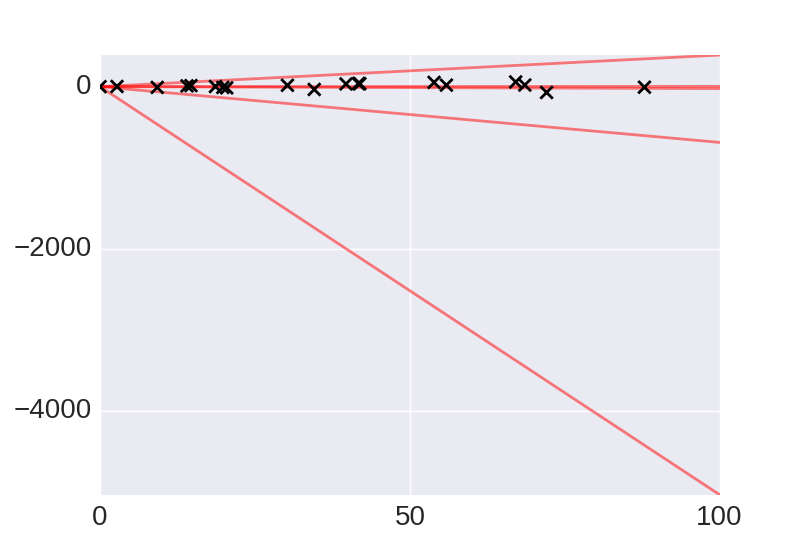
\includegraphics[width=\textwidth]{figs/composition/composition_demo_LIN_prior.png}
        \caption{LIN}
    \end{subfigure}
    ~ %add desired spacing between images, e. g. ~, \quad, \qquad, \hfill etc. 
      %(or a blank line to force the subfigure onto a new line)
    \begin{subfigure}[b]{0.3\textwidth}
        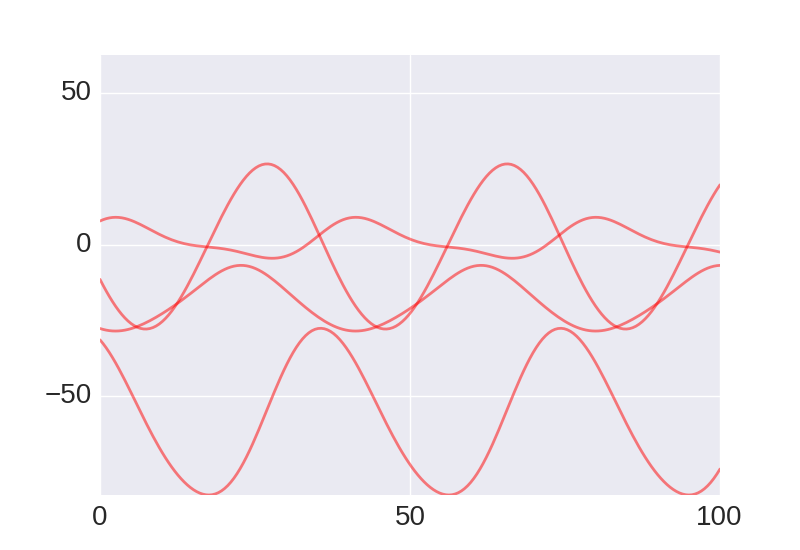
\includegraphics[width=\textwidth]{figs/composition/composition_demo_PER_prior.png}
        \caption{PER}
    \end{subfigure}
    ~ %add desired spacing between images, e. g. ~, \quad, \qquad, \hfill etc. 
    %(or a blank line to force the subfigure onto a new line)
    \begin{subfigure}[b]{0.3\textwidth}
        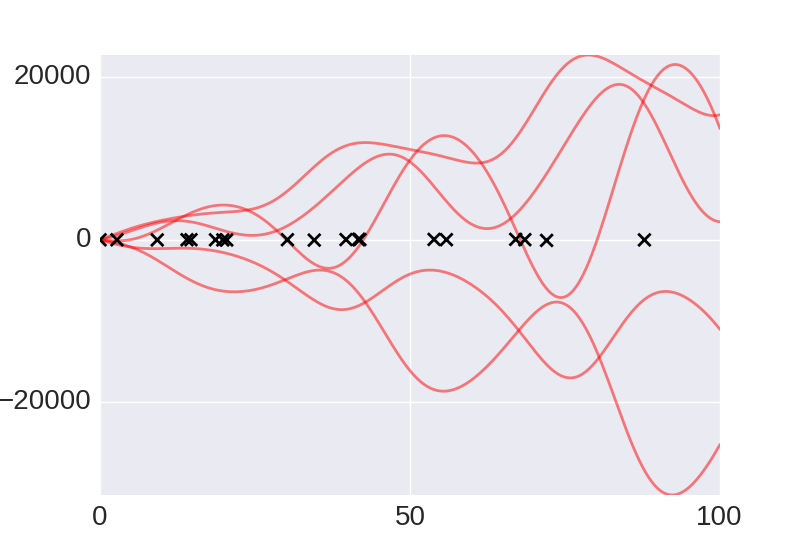
\includegraphics[width=\textwidth]{figs/composition/composition_demo_LINxPER_prior.png}
        \caption{LIN $\times$ PER}
    \end{subfigure} \vspace{4mm} 

Posterior:

 \begin{subfigure}[b]{0.3\textwidth}
        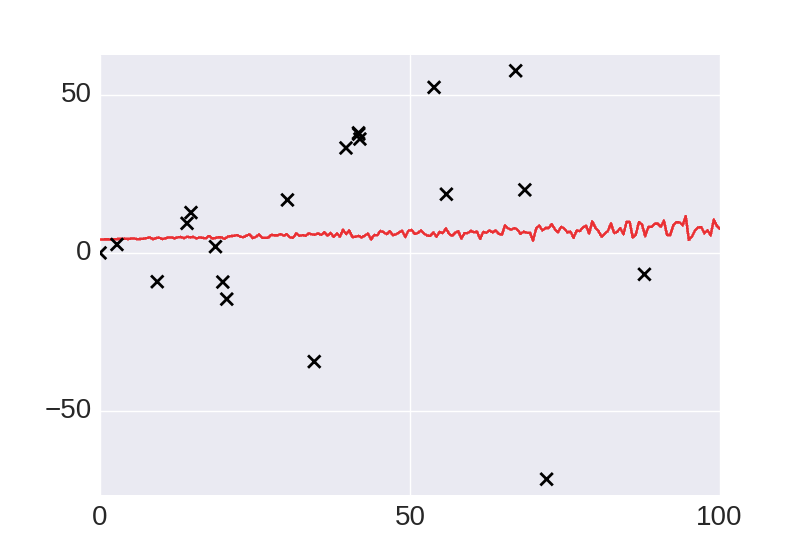
\includegraphics[width=\textwidth]{figs/composition/composition_demo_LIN.png}
        \caption{LIN}
    \end{subfigure}
    ~ %add desired spacing between images, e. g. ~, \quad, \qquad, \hfill etc. 
      %(or a blank line to force the subfigure onto a new line)
    \begin{subfigure}[b]{0.3\textwidth}
        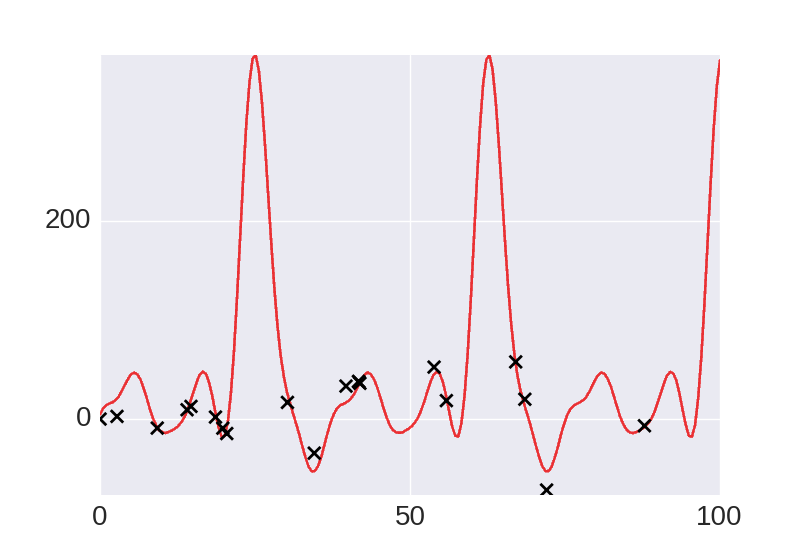
\includegraphics[width=\textwidth]{figs/composition/composition_demo_PER.png}
        \caption{PER}
    \end{subfigure}
    ~ %add desired spacing between images, e. g. ~, \quad, \qquad, \hfill etc. 
    %(or a blank line to force the subfigure onto a new line)
    \begin{subfigure}[b]{0.3\textwidth}
        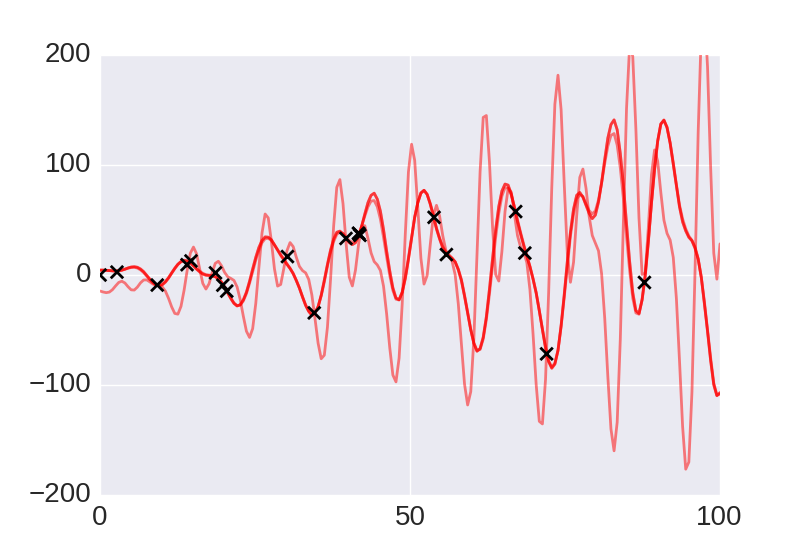
\includegraphics[width=\textwidth]{figs/composition/composition_demo_LINxPER.png}
        \caption{LIN $\times$ PER}
    \end{subfigure}

%20.0739791735
%6.31647597198
%37.7184218042
%19.1051376016

\caption{\footnotesize We depict kernel composition. 
(a) shows raw data (black) generated with a sine function with linearly growing amplitude (blue).
This data is used for all the plots (c-h). 
(b) shows the linear and the periodic base kernel in functional form as well as a composition of both. 
The multiplication of the two kernels indicates local interaction. The local interaction we account for in this case is the growing amplitude (a). For each column (c-h) $\bm{\theta}$ is different.(c-e) show samples from the prior
predictive $\ystar$ where random parameters are used, that is, we sample before any data points are observed.
(f-h) show samples from the predictive posterior $\yprime$, after the data has been observed.}
\label{fig:composition_tutorial}
\end{figure}
%%%%%%%%%%%%%%%%%%%%%%%%%%%%%%%%%%%%%%%%%%%%%%%%%%%%%%%%%%%%
These high-level properties are compositional via addition and multiplication of different covariance functions. 
That means that we can also combine these properties.
By using multiplication of kernels we can model a local interaction of two components, for example 
%%%%%%%%%%%%%%%%%%%%%%%%%%%%%%%%%%%%%%%%%%%%%%%%%%%%%%%%%%%%
\begin{equation}\label{eq:LINxPER}
    \klin \times \kper =  \sigma_1^2(x x^\prime)\, \sigma_2^2 \exp \bigg(
\frac{2 \sin^2 ( \pi (x - x^\prime)/p}{\ell^2} \bigg).
\end{equation}
%%%%%%%%%%%%%%%%%%%%%%%%%%%%%%%%%%%%%%%%%%%%%%%%%%%%%%%%%%%%
This results in a combination of the higher level properties of linearity and  periodicity.
In Fig \ref{fig:composition_tutorial} (e) we depict samples for $\ystar$ that are periodic
with linearly increasing amplitude.
We consider this a local interaction because the actual interaction depends on the similarity
of two data points.
An addition of covariance functions models a global interaction, that is an interaction of two high-level components that is qualitatively not dependent on the input space. An example for this a periodic function with a linear
trend.

For each kernel type, each $\bm{\theta}$ is different, that is, in (\ref{eq:LIN1}) we have $\thetabf=\{\sigma_1\}$,
in (\ref{eq:PER1}) we have $\bm{\theta}=\{\sigma_2,p,\ell\}$ and in 
(\ref{eq:LINxPER}) we have $\bm{\theta}=\{\sigma_1,\sigma_2,p,\ell\}$.
Adjusting these hyper-parameters changes lower level qualitative attributes such as length
scales ($\ell$) while preserving the higher level qualitative properties of the distribution
such as linearity. 



If we choose a suitable set of hyper-parameters, for example by performing inference, we
can capture the underlying dynamics of the data well (see Fig.
\ref{fig:composition_tutorial} (f-h)) while sampling $\yprime$.
Note that goodness of fit is not only limited to the parameters. A too simple qualitative structure
implies unsuitable behaviour, as for example in (Fig. \ref{fig:composition_tutorial} (g)) where additional 
recurring spikes are introduced to account for the changing amplitude of the true function that 
generated the data.





